%===================================================
%导论
\section  {INTRODUCTION}

%\section*{不编号的章节标题}
%\addcontentsline{toc}{INTRODUCTION}{不编号的章节标题}
%-------------------------------------------------
%问题重定义
\subsection{Problem Analysis}
\par
\lettrine[lines=2]{T}{oday},information has many channels to spread and to be recieved. 

\par Specifically, we face five subproblems:
\begin{itemize}
\item Develop one or more model(s) to explore the flow of information and filter;
\item Validate the models' reliability by using data from the past and the prediction capability of the model to predict the information communication situation for today and compare that with today's reality;
\item Use the model to predict the communication networks' relationships and capacities around the year 2050;

\item Use the theories and concepts of information influence on networks to model how public interest and opinion can be changed through information networks in today's connected world;

\item Determine how information value, people's initial opinion and bias, form of the message or its source, and the topology or strength of the information network in a region, country, or the world could be used to spread information and influence public opinion. 
\end{itemize}



 %-------------------------------------------------
 \subsection{Our work}

 
 \par We consider that the problems are progressive , which contributes to solve the main problem. To analyze the relationship between speed/flow of information versus inherent value of information of 5 periods and solve all problems, we should firstly know the basic definitions and how dissemination work. Then, we should make clear its development over time relative to its scale, spreading speed and impact. Subsequently, we discuss how to changed people's mind through the Internet and how the dissemination of information. Finally, we make a brief conclusion of models, apply them to some "What if" problems and summarize the whole passage.
 
 
%===================================================
%假设和参数


%===================================================
%问题分析


\section  {Assumptions}
\begin{itemize}
	\item Three roles take part in the dissemination of news:source, media and individual.
	\item Different types of roles' impact vary from one from another, while in a same type, different nodes' impact vary from one to another.
	\item The dissemination of information is with randomicity.
	\item The size of a node shows its impact.
	\item A line represents a two-way propagation. Each time, the direction of propagation depends on which node has greater influence.
\end{itemize}

%----------数据分析-----------
\section  {Data Analysis}

%----------问题1-----------
\section{Problem 1} 
\subsection{Assumptions}
\begin{itemize}
	\item Three roles take part in the dissemination of news:source, media and individual.
	\item Different types of roles' impact vary from one from another, while in a same type, different nodes' impact vary from one to another.
	\item The dissemination of information is with randomicity.
	\item The size of a node shows its impact.
	\item A line represents a two-way propagation. Each time, the direction of propagation depends on which node has greater influence.
\end{itemize}

\subsection{Model1}
\subsubsection*{Analyse}
\par The WS model in Small-world Network and the BA model Scale-free Network partly reveal some features of a network of communication such as its topology.
\par The WS Model emphasizes the relationship of pairs of nodes and their reconnections. 

\subsubsection*{Model Establishment}
\subsubsection*{Verification}
\subsection{The Results}

%----------问题2-----------
\section{Problem 2} 
\subsection{Assumptions}
\begin{itemize}
	\item Three roles take part in the dissemination of news:source, media and individual.
	\item Different types of roles' impact vary from one from another, while in a same type, different nodes' impact vary from one to another.
	\item The dissemination of information is with randomicity.
	\item The size of a node shows its impact.
	\item A line represents a two-way propagation. Each time, the direction of propagation depends on which node has greater influence.
\end{itemize}

\subsection{Model1}
\subsubsection*{Analyse}
\par The WS model in Small-world Network and the BA model Scale-free Network partly reveal some features of a network of communication such as its topology.
\par The WS Model emphasizes the relationship of pairs of nodes and their reconnections. To show the randomness, the WS Model add its paths randomly to a previous one, and derive as NW Model. The degree of nodes are similar due to its building way. Unfortunately, its nodes will never increase by time and each added path doesn't have any preference. That is, we can consider all nodes in a same scale in this model actually.  

\par The BA Model pays attention on a "preferable" 
\subsubsection*{Model Establishment}
\subsubsection*{Verification}
\begin{itemize}
	\item[-] $N$ :The number of factors.
	\item[-] $m$ :The number of periods.
	\item[-] $n$ :The length of time.
\end{itemize}

\par A raw fuction is:
\[
y=\frac{1}{K+ab^{t} }  \eqno (10)
\]
where
\[
K>0,a>0,0<b\neq 1
\]
Then,
\[y_{t}^{'}=K+ab^{t}\eqno (11)\]
We thus obtained their arguments from:
\[\left\{\begin{matrix}
&b=&\left ( \frac{S_{3}-S_{2}}{S_{2}-S_{1}} \right )^{\frac{1}{m}}   \\ 
&a=&(S_{2}-S_{1})\frac{b-1}{b\left ( b^{m}-1 \right )^{2}} \\
&  K=&\frac{1}{m}
\end{matrix}\right.\eqno (12)
\]
where\[S_{1}=\sum_{t=1}^{m}y^{'}_{t},S_{2}=\sum_{t=m+1}^{2m}y^{'}_{t},
S_{3}=\sum_{t=2m+1}^{3m}y^{'}_{t}\eqno(13)\]
	\par In this model, we consider five periods from 1920s to 2010s. $n$ is $90$ while $m$ is $5$.




\begin{figure}[h]
	\small
	\centering
	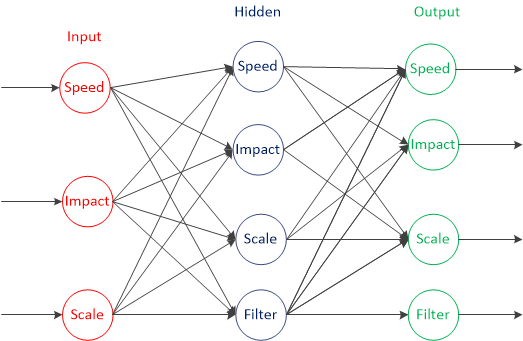
\includegraphics[width=12cm]{./picture/BPm.png}
	\caption{A initial BP Model}
	 \label{fig:A initial BP Model}
\end{figure}
In this model, some parameters can be defined as:
\[input=\sum_{i=1}^{3}input(i)\eqno(21)\]
\[hidden:n=\sqrt{\sum_{i=1}^{3}input(i)+4}\eqno(22)\]
where $i$ is shenjingyuanshuliang.
\[output(j)=\sum_{j=1}^{4}func\left ( n \right )\eqno(23)\]
where $func(x)$ is a function calculating the influence of $n$.


\subsection{The Results}


	\par We access some data from the Internet and make the average value as shown below:
\begin{table}[tbp]
	 \centering% 表居中
	\begin{tabular}{lccccc}  % {lccc} 表示各列元素对齐方式,left-l,right-r,center-c
		\hline
		Items & 1870s & 1920s & 1970s & 1990s & 2010s\\ \hline  % \hline 在此行下面画一横线
		RI (years) & 80 & 70  & 50  & 20 & 20 \\         % \\ 表示重新开始一行
		OS (hours)& 72 & 5 & 2 & 0.5 & 0.17\\        % & 表示列的分隔线
		RS (hours) & 158 & 48 & 24 & 3 & 0.5\\ 
		RT (hours) & 42 & 65 & 112 & 158 & 187  \\
		\hline
	\end{tabular}
	\caption{Data obtained through the Internet}\label{tab:1}
\end{table} 
\par Then ,we put them into our modified model, and get the result as:
\begin{figure}[h]
	\small
	\centering
	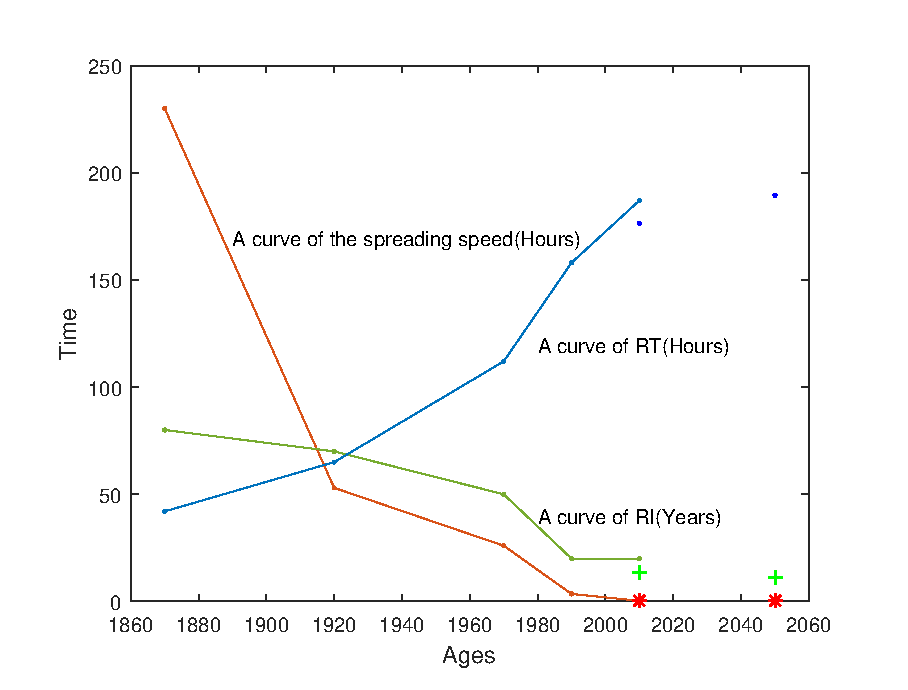
\includegraphics[width=15cm]{./picture/wtf.eps}
	\caption{The results}
	\label{fig:The results}
\end{figure}

\par Where the solid line the real data and the singles points are generated by the modified model.

\begin{table}
	\centering% 表居中
	\begin{tabular}{lccccc}  % {lccc} 表示各列元素对齐方式,left-l,right-r,center-c
		\hline
		Items & MSE & SSE   & RMSE\\ \hline  % \hline 在此行下面画一横线
		RI   & 40.4496  & 40.4496  & 6.3600 \\         % \\ 表示重新开始一行
		SS (hours)& 0.0121  & 0.0121 & 0.1100 \\        % & 表示列的分隔线
		RT (hours) & 111.7249 & 111.7249 & 10.5700   \\
		\hline
	\end{tabular}
	\caption{Data through the Internet}\label{tab:1}
\end{table} 
\par To confirm its capability of predicting, we use the $MSE,SSE,RMSE$ to measure the prediction model. The measure of the prediction error is shown in $Table 2$. As a matter of fact it doesn't seem to work,it tells nothing. We consider it's a result of the poor scale of data.
\subsection*{Extends}
\par Refer to the impact a dissemination network brings, we should consider in different periods, different devices show them in different ways. We find some data which reveals the impact of different periods of different devices as below:




\section{CONCLUSIONS}
%============================模型=优点====================================
\subsubsection*{Strengths}
\begin{itemize}
	\item {Applies widely}
	\item \textbf{The models possess practicability and value of popularization}
	\item {From the perspective of as many as possible }
	\item {The models are simple and easy to understand}
	\item {Some of the ideas are very new}
\end{itemize}
\subsubsection*{Weakness}
\begin{itemize}
	\item {The models reveal subjectivity to a certain extent}
	\item {Model in the primary stage}
	\item {Many factors are not considered }
	\item {Some calculating principles have not been explain clearly}
	\item {Few data can be put into testing}
	
\end{itemize}
%======================================================================
\subsection{Summary}



\begin{thebibliography}{99}
	
%\addcontentsline{toc}{section}{References}
\bibitem{1}David A. Freedman (2009). Statistical Models: Theory and Practice. Cambridge University Press. p. 128
\bibitem{2}Walker, SH; Duncan, DB (1967). "Estimation of the probability of an event as a function of several independent variables". Biometrika 54: 167-178. doi:10.2307/2333860
\bibitem{3} Saaty, Thomas L.; Peniwati, Kirti (2008). Group Decision Making: Drawing out and Reconciling Differences. Pittsburgh, Pennsylvania: RWS Publications. ISBN 978-1-888603-08-8
\bibitem{4}Watts, Duncan J.; Strogatz, Steven H. (June 1998). "Collective dynamics of 'small - world' networks". Nature 393 (6684): 440 - 442. 
\bibitem{5}Onnela, J. -P.; Saramaki, J.; Hyvonen, J.; Szabo, G.; Lazer, D.; Kaski, K.; Kertesz, J.; Barabasi, A. -L. (2007). "Structure and tie strengths in mobile communication networks". Proceedings of the National Academy of Sciences 104 (18): 7332-7336
\bibitem{6}Choromański, K.; Matuszak, M.; MiȩKisz, J. (2013). "Scale-Free Graph with Preferential Attachment and Evolving Internal Vertex Structure". Journal of Statistical Physics 151 (6): 1175.

\bibitem{7}Moonchai S, Rakpuang W. A New Approach to Improve Accuracy of Grey Model GMC in Time Series Prediction[J]. Modelling and Simulation in Engineering, 2015, 2015.
\bibitem{8}Hou S Q. Forecasting of Water Resource of China based on Grey Prediction Model[J]. Advance Journal of Food Science and Technology, 2015, 9(5): 389-392.

\bibitem{9}
Saracoglu, B.O. (2013). "Selecting industrial investment locations in master plans of countries". European J. of Industrial Engineering (Inderscience Enterprises Ltd.) 7 (4): 416-441. doi:10.1504/EJIE.2013.055016
\bibitem{10}He Y, Li X, Deng X. Discrimination of varieties of tea using near infrared spectroscopy by principal component analysis and BP model[J]. Journal of Food Engineering, 2007, 79(4): 1238-1242.
\bibitem{11}http://www.people-press.org/2012/09/27/section-1-watching-reading-and-listening-to-the-news-3/
\bibitem{12}http://www.nature.com/nature/journal/v393/n6684/full/393440a0.html
\bibitem{13}
https://en.wikipedia.org/wiki/Principalcomponentanalysis
\bibitem{14}
https://en.wikipedia.org/wiki/Analytichierarchyprocess 

\bibitem{15}https://en.wikipedia.org/wiki/Scale-free-network
\bibitem{16}https://en.wikipedia.org/wiki/Small-world-network
\bibitem{17}https://en.wikipedia.org/wiki/Logistic-regression
\bibitem{18}https://en.wikipedia.org/wiki/Artificial-neural-network
\bibitem{19}http://baike.baidu.com/link?url=Qm-xihbLpYtYMbmzQZGTX9wSVvMSL4lpL7nto1PFVJ2wiGCKMaDMnQ1WORkeY8aqpaCvBE1m5aMq2zkR8xM0FK
\end{thebibliography}

%====================附录导入程序代码==========================================
\begin{appendices}
   
\textbf{\textcolor[rgb]{0.98,0.00,0.00}{The core codes of the BP Model:}}
\lstinputlisting[language=Matlab]{./code/matlab1.m}


\textbf{\textcolor[rgb]{0.98,0.00,0.00}{The core codes of Grey Prediction model,GM(1,n):}}
\lstinputlisting[language=Matlab]{./code/huise_gm1n.m}
\end{appendices}
